\chapter{Deuteronomy 13}

\begin{figure}
  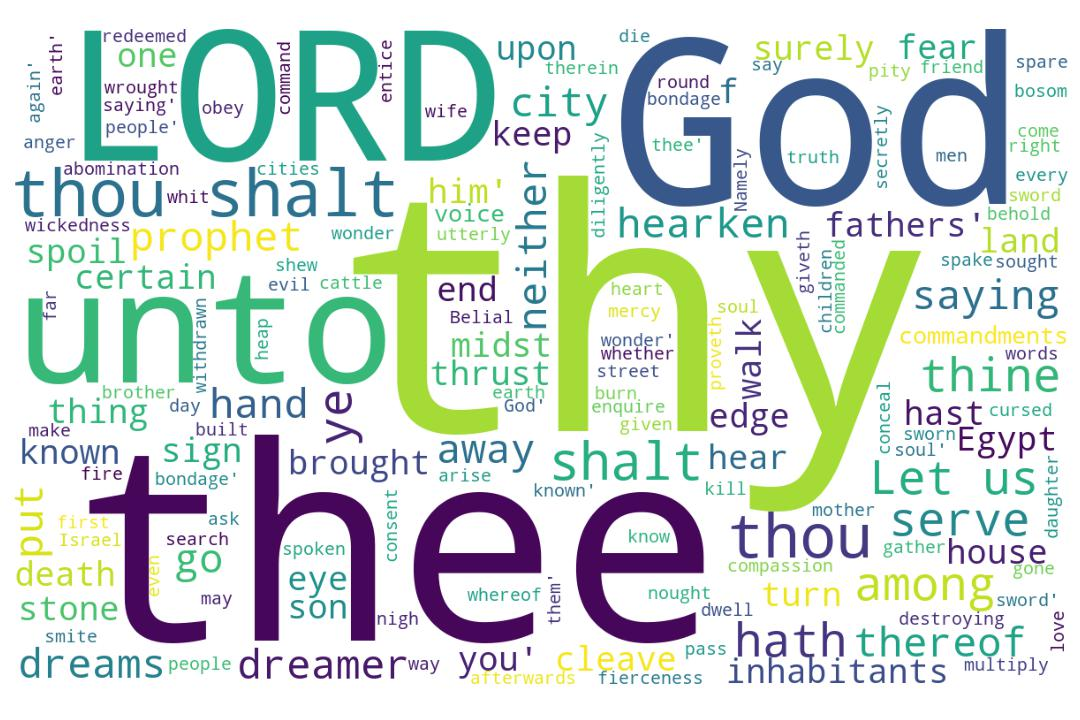
\includegraphics[width=\linewidth]{05OT-Deuteronomy/Deuteronomy13-WordCloud.jpg}
  \caption{Deuteronomy 13 Word Cloud}
  \label{fig:Deuteronomy 13 word Cloud}
\end{figure}

\marginpar{\scriptsize \centering \fcolorbox{bone}{lime}{\textbf{STAY TRUE}}\\ (Deuteronomy 13:1-22) \begin{compactenum}[I.][8]
    \item  A \textbf{Prophet with Signs }  \index[scripture]{Deuteronomy!Deu 13:01} \index[scripture]{Deuteronomy!Deu 13:03}\index[scripture]{Deuteronomy!Deu 13:05}(Deu 13:1, 3, 5)
    \item  The \textbf{Proof  of Sincerity}  \index[scripture]{Deuteronomy!Deu 13:03} (Deu 13:3)
    \item   \textbf{People gone Sideways}  \index[scripture]{Deuteronomy!Deu 13:07}\index[scripture]{Deuteronomy!Deu 13:09} (Deu 13:7, 9)
    \item   No \textbf{Pity or Sparing}  \index[scripture]{Deuteronomy!Deu 13:08}(Deu 13:8)
    \item   The \textbf{Pull to false Service}  \index[scripture]{Deuteronomy!Deu 13:13}(Deu 13:13)
    \item    \textbf{Punishment with Swords}  \index[scripture]{Deuteronomy!Deu 13:15}(Deu 13:15)
    \item    \textbf{Purging the Spoil}  \index[scripture]{Deuteronomy!Deu 13:16}(Deu 13:16)
\end{compactenum}}



\footnote{\textcolor[cmyk]{0.99998,1,0,0}{\hyperlink{TOC}{Return to end of Table of Contents.}}}\footnote{\href{https://audiobible.com/bible/deuteronomy_13.html}{\textcolor[cmyk]{0.99998,1,0,0}{Deuteronomy 13 Audio}}}\textcolor[cmyk]{0.99998,1,0,0}{If there arise among you \fcolorbox{bone}{lime}{a prophet}, or a dreamer of dreams, and giveth thee a sign or a wonder,}
[2] \textcolor[cmyk]{0.99998,1,0,0}{And the sign or the wonder come to pass, whereof he spake unto thee, saying, Let us go after other gods, which thou hast not known, and let us serve them;}
[3] \textcolor[cmyk]{0.99998,1,0,0}{Thou \fcolorbox{bone}{bone}{shalt} not hearken unto the words of that \fcolorbox{bone}{lime}{prophet}, or that dreamer of dreams: for the LORD your God \fcolorbox{bone}{lime}{proveth} you, to know whether ye love the LORD your God with all your heart and with all your soul.}
[4] \textcolor[cmyk]{0.99998,1,0,0}{Ye shall walk after the LORD your God, and fear him, and keep his commandments, and obey his voice, and ye shall serve him, and cleave unto him.}
[5] \textcolor[cmyk]{0.99998,1,0,0}{And that \fcolorbox{bone}{lime}{prophet}, or that dreamer of dreams, shall be put to death; because he hath spoken to turn \emph{you} away from the LORD your God, which brought you out of the land of Egypt, and redeemed you out of the house of bondage, to thrust thee out of the way which the LORD thy God commanded thee to walk in. So \fcolorbox{bone}{bone}{shalt} thou put the evil away from the midst of thee.}\\
\\
\P \textcolor[cmyk]{0.99998,1,0,0}{If thy brother, the son of thy mother, or thy son, or thy daughter, or the wife of thy bosom, or thy friend, which \emph{is} as thine own soul, entice thee secretly, saying, Let us go and serve other gods, which thou hast not known, thou, nor thy fathers;}
[7] \textcolor[cmyk]{0.99998,1,0,0}{\emph{Namely}, of the gods of the people which \emph{are} round about you, nigh unto thee, or far off from thee, from the \emph{one} end of the earth even unto the \emph{other} end of the earth;}
[8] \textcolor[cmyk]{0.99998,1,0,0}{Thou \fcolorbox{bone}{bone}{shalt} not consent unto him, nor hearken unto him; neither shall thine eye \fcolorbox{bone}{lime}{pity} him, neither \fcolorbox{bone}{bone}{shalt} thou spare, neither \fcolorbox{bone}{bone}{shalt} thou conceal him:}
[9] \textcolor[cmyk]{0.99998,1,0,0}{But thou \fcolorbox{bone}{bone}{shalt} surely kill him; thine hand shall be first upon him to put him to death, and afterwards the hand of all the people.}
[10] \textcolor[cmyk]{0.99998,1,0,0}{And thou \fcolorbox{bone}{bone}{shalt} stone him with stones, that he die; because he hath sought to thrust thee away from the LORD thy God, which brought thee out of the land of Egypt, from the house of bondage.}
[11] \textcolor[cmyk]{0.99998,1,0,0}{And all Israel shall hear, and fear, and shall do no more any such wickedness as this is among you.}\\
\\
\P \textcolor[cmyk]{0.99998,1,0,0}{If thou \fcolorbox{bone}{bone}{shalt} hear \emph{say} in one of thy cities, which the LORD thy God hath given thee to dwell there, saying,}
[13] \textcolor[cmyk]{0.99998,1,0,0}{\emph{Certain} men, the children of Belial, are gone out from among you, and have withdrawn the inhabitants of their city, saying, Let us go and serve other gods, which ye have not known;}
[14] \textcolor[cmyk]{0.99998,1,0,0}{Then \fcolorbox{bone}{bone}{shalt} thou enquire, and make search, and ask diligently; and, behold, \emph{if} \emph{it} \emph{be} truth, \emph{and} the thing certain, \emph{that} such abomination is wrought among you;}
[15] \textcolor[cmyk]{0.99998,1,0,0}{Thou \fcolorbox{bone}{bone}{shalt} surely smite the inhabitants of that city with the edge of the \fcolorbox{bone}{lime}{sword}, destroying it utterly, and all that \emph{is} therein, and the cattle thereof, with the edge of the sword.}
[16] \textcolor[cmyk]{0.99998,1,0,0}{And thou \fcolorbox{bone}{bone}{shalt} gather all the \fcolorbox{bone}{lime}{spoil} of it into the midst of the street thereof, and \fcolorbox{bone}{bone}{shalt} burn with fire the city, and all the \fcolorbox{bone}{lime}{spoil} thereof every whit, for the LORD thy God: and it shall be an heap for ever; it shall not be built again.}
[17] \textcolor[cmyk]{0.99998,1,0,0}{And there shall cleave nought of the cursed thing to thine hand: that the LORD may turn from the fierceness of his anger, and shew thee mercy, and have compassion upon thee, and multiply thee, as he hath sworn unto thy fathers;}
[18] \textcolor[cmyk]{0.99998,1,0,0}{When thou \fcolorbox{bone}{bone}{shalt} hearken to the voice of the LORD thy God, to keep all his commandments which I command thee this day, to do \emph{that} \emph{which} \emph{is} right in the eyes of the LORD thy God.}